\chapter{Deep Learning Fundamentals}

\section{Artificial Neural Networks}

Artificial neural networks (ANNs) are a class of machine learning algorithms
that are loosely inspired by the structure of biological nervous
systems.
To be precise, each ANN consists of a collection of artificial neurons
that are connected with each other. The neurons are able to exchange
information along their connections.
A common way to arrange artificial neurons within a network is to organize
them in layers as depicted in \fref{fig:basic-network}.
\begin{figure}[h]
  \centering
  \resizebox{0.75\textwidth}{!}{\begin{neuralnetwork}[height=5]
  \tikzstyle{input neuron}=[neuron, draw, fill=white]
  \tikzstyle{hidden neuron}=[neuron, draw, fill=white]
  \tikzstyle{output neuron}=[neuron, draw, fill=white]
  \tikzstyle{link} = [->, shorten <=0pt, node distance=\nn@layerspacing, thin, draw=black];
  \inputlayer[count=4, bias=false, title=Input\\layer]
  \hiddenlayer[count=5, bias=false, title=Hidden\\layer] \linklayers
  \outputlayer[count=3, title=Output\\layer] \linklayers
\end{neuralnetwork}
}
  \caption{The structure of an ANN can be described by a
    directed graph. The nodes represent the
    neurons, the edges represent their connections, also indicating
    the flow of information.}
  \label{fig:basic-network}
\end{figure}

When an artificial neuron receives signals on some of its
incoming connections, it may elect to become active based on the input
it collects.\footnote{The
  details of this
  process are further illustrated in \fref{sec:artificial-neurons}.}
In this state it also influences all neurons it has an outgoing
connection to by passing a signal along their
channel. Those other neurons in turn may also elect to become
active - this way a signal can propagate through the network along
the connecting edges.

Usually, each ANN consists of at least one layer of neurons that is
responsible for receiving signals from the environment - we call this
an \textit{input layer} (see \fref{fig:basic-network}). When these neurons
receive a signal from the environment, they propagate it to their
connected neighbors in the next layer. This process repeats until the
\textit{output layer} is reached. The neurons in this layer represent the
output of the whole network. Each layer in between is called a \textit{hidden
layer} because there is no direct communication between the neurons in
this layer and the environment. Networks that satisfy this basic
architectural model where each layer is fully connected with its
following layer and signals only flow in one direction without cycles
are called
\textit{fully connected feedforward networks}.

The goal behind this procedure usually is to convert an input signal
into a meaningful output by feeding it through the network. If the
network is able to detect relevant features or patterns in the input
signal, it can be used to perform tasks such as classification or
regression (i.e. approximate discrete or continuous functions).
In order for this to be possible, some kind of learning has to take
place which enables the network to capture the essence of the data it
is confronted with. We will take a further look at these aspects as
well as the mathematical model of a neural network in the following
sections.

\subsection{Modeling Artificial Neurons}
\label{sec:artificial-neurons}
To fully understand how each neuron processes the signals it receives,
it is necessary to develop a mathematical model that describes all the
operations taking place. The following descriptions are partially
based on the explanations that are provided in \cite{Haykin}.\footnote{See
  chapter I.3: \textit{Models of a Neuron} for more details.}
As shown in \fref{fig:single-neuron}, each artificial neuron
basically consists of three components:
\begin{enumerate}
  \item \textbf{A set of weighted inputs:} Each connection that is
    leading into the neuron has a weight \(w_{kj}\) associated with it
    where \(k\) denotes the neuron in question and \(j\) denotes the
    index of the neuron that delivers its input to the current neuron
    \(k\).\footnote{There might arise the question why the indexing of
    a weight from neuron \(j\) to neuron \(k\) is \(w_{kj}\) and
    \textit{not} \(w_{jk}\). This is the case because the weights are
    usually stored in matrices where each row corresponds to a
    neuron \(k\) and each column corresponds to an input \(j\) which
    allows for much faster computations by heavily utilizing
    matrix-multiplication.} The signal that
    passes the connection is multiplied by the
    related weight of that connection before arriving at the next
    component.
  \item \textbf{A summation unit:} This component adds up all the
    weighted signals that arrive at the neuron as well as a constant
    bias value
    \(b_k\) that is independent of the inputs. The reason for adding
    the bias term is explained in \fref{sec:bias}.
  \item \textbf{An activation function:} The activation function
    \(\phi(\cdot)\) applies a transformation to the output of the
    summation unit that is usually non-linear. The value of
    the activation function is the output of the neuron which will
    travel further through the network alongside the corresponding
    connections. In \fref{sec:activation-functions}, a more
    detailed explanation of activation functions as well as some
    commonly used examples will be provided.
\end{enumerate}
\begin{figure}[h]
  \centering
  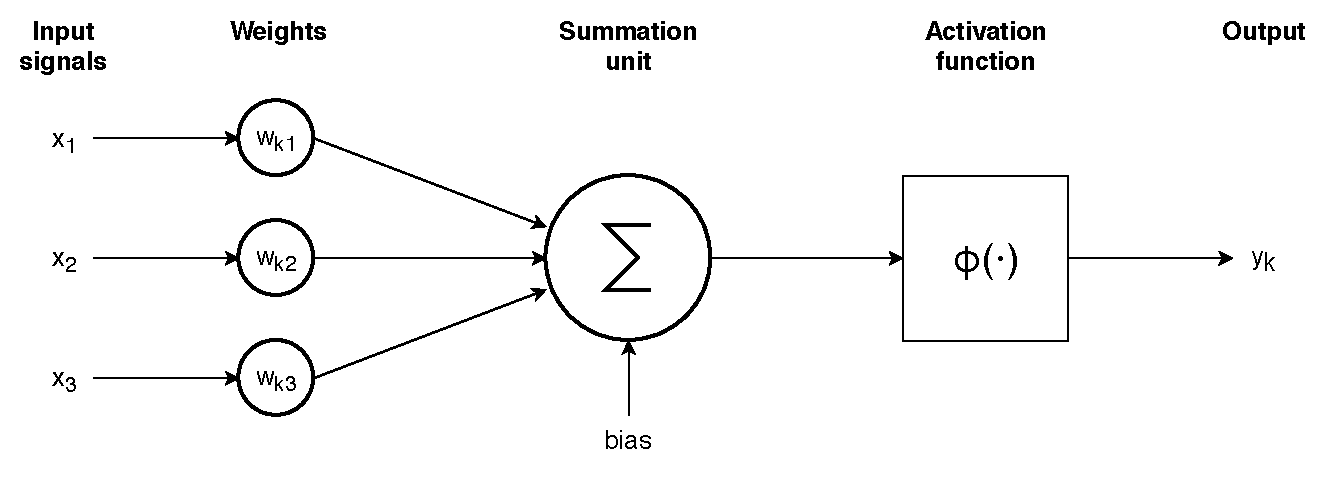
\includegraphics[width=\textwidth]{../figures/single_neuron}
  \caption{The components of a single artificial neuron. This neuron
    \(k\) receives three input signals that are first multiplied by
    the associated weights, summed up including a bias and then fed
    into an activation function that will determine the ouput signal.}
  \label{fig:single-neuron}
\end{figure}
Transforming this model into mathematical equations, the output of the
summation unit of a particular
neuron \(k\) with \(n\) input signals \(x_j\) can be described by the
following formula:
\begin{equation}
  \label{eq:input}
  z_k = \sum_{j=1}^{n}{x_j \cdot w_{kj}} + b_k
\end{equation}
where \(b_k\) denotes the bias term of neuron \(k\) and \(z_k\) describes the
result of the summation unit.

As a consequence, the output signal \(y_k\) of neuron \(k\) can be computed by
applying the activation function \(\phi(\cdot)\) to the output of the
summation unit which can be described by the following expression:
\begin{equation}
  y_k = \phi(z_k)
\end{equation}

\subsection{Activation Functions}
\label{sec:activation-functions}
The basic task of an activation function is to determine the level of
activity that a neuron emits based on the input it receives. Because the
incoming signals are first weighted and summed up by the summation unit, they
arrive at the activation function as a single value \(z\). Since the
output \(y\)
of the neuron is also a scalar, each activation function can be
described as \(\phi: \mathbb{R} \rightarrow \mathbb{R}\). In the
following paragraphs, an overview of the most popular activation
functions will be presented that is based on the descriptions found in
\cite{Patterson}.\footnote{See section \textit{Activation Functions}
  in chapter two.}

\paragraph{The Sigmoid Function}
\label{sec:sigmoid}
This activation function transforms an input \(z\) into a range between 0
and 1 based on the following equation:
\begin{equation}
  \phi(z) = \frac{1}{1 + e^{-\theta \cdot z}}
\end{equation}
The \(\theta\) parameter is used to adjust the sensitivity of the
sigmoid function with respect to its input signal. High values of \(\theta\) lead
to steep slopes around \(z=0\) while smaller values will lead to smoother
slopes. An illustration of this relationship is presented in \fref{fig:sigmoid}.
\begin{figure}[h]
  \centering
  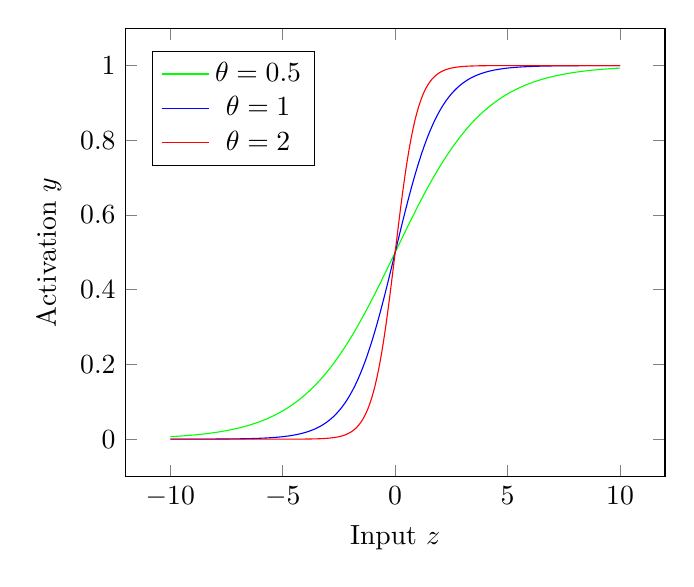
\begin{tikzpicture}
  \begin{axis}[
      xlabel={Input \(z\)},
      ylabel={Activation \(y\)},
      legend style={
        at={(0.05, 0.95)},
        anchor=north west
      }
    ]
    \addplot[green, domain=-10:10, samples=400]{1/(1+exp(-0.5*x))};
    \addplot[blue, domain=-10:10, samples=400]{1/(1+exp(-x))};
    \addplot[red, domain=-10:10, samples=400]{1/(1+exp(-2*x))};
    \legend{\(\theta = 0.5\), \(\theta = 1\), \(\theta = 2\)}
  \end{axis}
\end{tikzpicture}

  \caption{The sigmoid activation function plotted for different
    values of \(\theta\).}
  \label{fig:sigmoid}
\end{figure}

One important reason why the sigmoid function is often used is that it reduces
the impact of outliers in the data without removing them. When the
input of a neuron is large, it is reduced to a number near one, when it
is very negative, the activation evaluates to a number near zero. This
behaviour adds to the overall robustness of the network.

\paragraph{The Rectified Linear Unit (ReLU)}
Because it is not always desirable to reduce large signals to a
smaller scale, this function will only replace negative values with
zero and leave positive values untouched. This behaviour can be
modeled by the following expression:
\begin{equation}
  \phi(z) = \max(0, z)
\end{equation}
When building deep neural networks, one of the problems that sometimes
arise is that a signal will fade out when propagating through many
hidden layers. This issue is remedied to some degree by using the ReLU
function because large signals are not cut down. Due to the negative
values being set to zero, the ReLU function is also non-linear when
taking its whole domain into account. This is an important concept
because non-linear activation functions are essential for a network to
learn complex relationships. Another benefit of the ReLU function is
that its derivative is either 1 or 0. This will turn out to be important when
looking into the training of a neural network. Because of all these benefits,
ReLUs are one of the state of the art activation functions in deep
neural networks. A plot of the ReLU function is presented in \fref{fig:relu}.
\begin{figure}[h]
  \centering
  \begin{tikzpicture}
  \begin{axis}[
      xlabel={Input \(z\)},
      ylabel={Activation \(y\)},
      legend style={
        at={(0.05, 0.95)},
        anchor=north west
      }
    ]
    \addplot[blue, domain=-10:10]{max(0, x)};
  \end{axis}
\end{tikzpicture}

  \caption{The ReLU activation function.}
  \label{fig:relu}
\end{figure}

\paragraph{The Softmax Activation Function}
\label{sec:softmax}
This activation function is usually applied to the output neurons of
a network. When a neural network is used to perform classification
tasks, each output neuron is commonly associated with a specific
class. In classification tasks it is highly desirable to assign a
probability to each class that represents how likely it is that the
input data belongs to that class. The softmax activation function is
used to achieve this by setting up the output neurons to represent a
probability distribution over all possible classes.
In an output layer consisting of \(n\) output neurons, the softmax
function for each neuron \(i\) of that layer can be described by the
following equation, where \(z_i\) denotes the summation units' output of
the \(i\)'th neuron:
\begin{equation}
  \phi(z_i) = \frac{e^{z_i}}{\sum_{j=1}^{n}{e^{z_j}}}
\end{equation}
The softmax activation function represents -- loosely speaking -- the
percentage of the current neurons activation with respect to the compound
activation of all neurons in the layer.

There might arise the question why each input \(z_i\) is first fed
into the exponential function \(e^x\) before translating the
activations into probabilities. This is done to further amplify the
strongest signals and attenuate the weaker ones which results in more
clear-cut values.\footnote{Imagine the \(z_i\) inputs of the output
  layer are given by the following vector: \((2, 4, 2, 1)^T\). If we
  just normalize these values to obtain a probability for each neuron,
  we get \((0.22, 0.44, 0.22, 0.11)^T\). Using the exponential
  function first, we roughly get \((0.1, 0.75, 0.1, 0.05)^T\) which
  amplifies the most likely outcomes and attenuates the less likely
  ones. See
  \url{https://datascience.stackexchange.com/questions/23159/in-softmax-classifier-why-use-exp-function-to-do-normalization}
  for a nice explanation and the source of this example.}

\subsection{The Role of the Bias Value}
\label{sec:bias}
There still remains the question why in each artificial neuron there
is a bias value \(b_k\) added to the weighted sum of the inputs. The
reason for this is related to the activation function: The bias term
acts like a parameter that determines how to shift the activation
function along the x-axis. We already know from \fref{eq:input} that
for a neuron \(k\) with \(n\) inputs the toal input signal \(z_k\)
adds up to:
\begin{equation*}
  z_k = \sum_{j=1}^{n}{x_j \cdot w_{kj}} + b_k
\end{equation*}
Let us denote the weighted sum of the input signals as a separate
value \(a_k = \sum_{j=1}^{n}{x_j \cdot w_{kj}}\) that describes the raw
input of the neuron. This means that \(z_k
= a_k + b_k\) and using the sigmoid function (see \fref{sec:sigmoid}) as an example to
demonstrate the effects of the bias value, we can slightly rewrite it as
\begin{equation*}
  \phi(a_k) = \frac{1}{1+e^{-(a_k+b_k)}}
\end{equation*}
also setting \(\theta = 1\) for demonstration purposes. Plotting the
activation function for
different values of \(b_k\) immediately reveals the effect of the bias
value as a shift-parameter which can be seen in \fref{fig:bias}.
\begin{figure}[h]
  \centering
  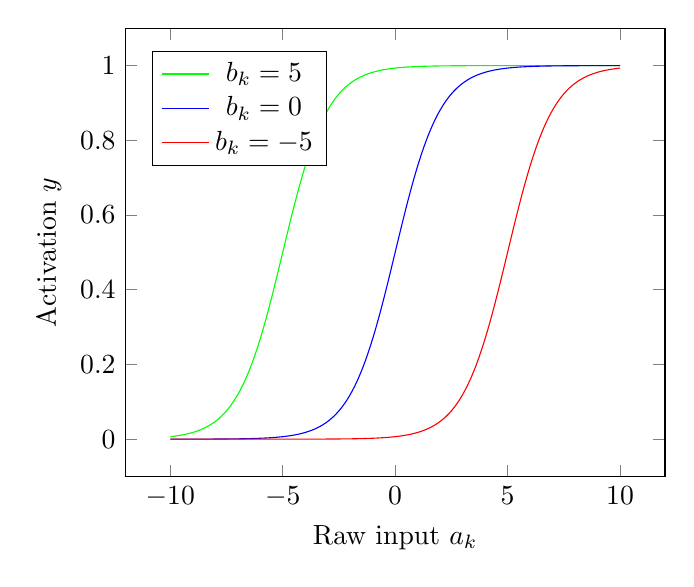
\begin{tikzpicture}
  \begin{axis}[
      xlabel={Raw input \(a_k\)},
      ylabel={Activation \(y\)},
      legend style={
        at={(0.05, 0.95)},
        anchor=north west
      }
    ]
    \addplot[green, domain=-10:10, samples=400]{1/(1+exp(-(x+5)))};
    \addplot[blue, domain=-10:10, samples=400]{1/(1+exp(-x))};
    \addplot[red, domain=-10:10, samples=400]{1/(1+exp(-(x-5)))};
    \legend{\(b_k = 5\), \(b_k = 0\), \(b_k = -5\)}
  \end{axis}
\end{tikzpicture}

  \caption{The sigmoid activation function plotted for different bias values.}
  \label{fig:bias}
\end{figure}

What this shift means is that the bias term acts like a threshold that
has to be overcome in order for the neuron to become active. Positive
bias values lead to activity even when the raw input \(a_k\) is still
negative and negative bias values require bigger input signals in
order for the neuron to fire.

\section{Neural Networks as Classifiers}

After establishing a mathematical model that helps us to describe a
neural network, there is still one problem to be solved: How to train
the network to be able to successfully perform tasks such as
classification? In order to figure this out, we will first take a look at
classification tasks in general and then explore how to set up and
train a neural network to perform classification.

\subsection{Classification}

The basis of a classification task is usually formed by a dataset that
consists of features as well as labels. The goal of the classification
algorithm is to predict the label of an instance of the dataset by
only looking at its features. In order to achieve this, the classifier
first has to build a model based on a training dataset. This procedure is called
\textit{training}. In the next step, the classifier is presented with
some new examples that it did not see during training. The classifier
is tested on these new examples to estimate its performance and to see
if it was able to learn any concepts from the data, i.e. to
\textit{generalize}. This phase is also
called \textit{testing}. Because classification requires pre-labeled
instances and the classifier acts like a learner who learns from a
teacher, classification is an example of a broader domain called
\textit{supervised learning}.

\subsubsection{Evaluating a Classifier}

In order to find out how well a classifier generalizes after training,
the results of the testing phase can be entered into a
\textit{confusion matrix} that is structured as shown in
\fref{fig:confusion-matrix}.\footnote{It should be noted that this
  concept can be
  extended to classification tasks with more than two classes as well
  by simply adding new rows and columns for each new class.}
\begin{figure}[h]
  \centering
  \renewcommand\theadfont{\bfseries}
  \begin{tabular}{|c|c|c|}
    \hline
    & \thead{Class Positive\\(Predicted)} & \thead{Class Negative\\(Predicted)} \\
    \hline
    \thead{Class Positive\\(Actual)} & True positives (TP) & False
    negatives (FN) \\
    \hline
    \thead{Class Negative\\(Actual)} & False positives (FP) & True
    negatives (TN) \\
    \hline
  \end{tabular}
  \caption{The structure of a confusion matrix for a
    classification task with two classes ``positive'' and
    ``negative''.}
  \label{fig:confusion-matrix}
\end{figure}

Each entry in this matrix describes how often the
classifier was presented with an example of the row-class during testing and
predicted that the example belongs to the column-class. The resulting
measurements of true positives, true negatives, false positives and
false negatives can be used to compute the following evaluation
metrics:\footnote{A collection of these metrics can also be found in
  \cite{Patterson}, see chapter \textit{Evaluating Models}.}

\paragraph{Accuracy} This measurement determines the percentage of
examples in the testing set that the classifier predicted correctly.
It can be denoted by the following equation:
\begin{equation}
  Accuracy = \frac{TP + TN}{TP + TN + FP + FN}
\end{equation}
This metric works well if there is roughly an equal amount of examples
for each class. However if one of the classes makes up most of the
examples, the classifier can reach a high degree of accuracy by just
predicting the label of the dominant class every single time. This
impairs the significance of this metric when imbalances among the
classes are present.

\paragraph{Precision} The precision score shows the percentage of
examples that were correctly classified as positive among all examples
that the classifier labeled positive:
\begin{equation}
  Precision = \frac{TP}{TP + FP}
\end{equation}
This metric can also be interpreted as an estimate of the conditional probability
that the classifier is right given that it predicted a positive class:
\begin{equation*}
  Precision = P(\text{Classifier is right} \vert \text{Classifier predicted
    POSITIVE})
\end{equation*}

\paragraph{Recall} This measurement remedies the imbalance issues of
the accuracy metric by determining the percentage of correctly
classified examples for each separate class. It can be denoted by the
following expression:
\begin{equation}
  Recall = \frac{TP}{TP + FN}
\end{equation}
The recall score can also be interpreted as an estimate of the conditional
probability that the
classifier is right given a specific class:
\begin{equation*}
  Recall = P(\text{Classifier is right} \vert \text{Class is POSITIVE})
\end{equation*}

\paragraph{F1 Score} This metric combines precision and recall to
calculate their so called \textit{harmonic mean}. It is often used
when evaluating classification models, thus its equation is also
displayed here:
\begin{equation}
  \text{F1 Score} = \frac{2*Precision*Recall}{Precision+Recall}
\end{equation}
\\
It should be noted that all these measurements can be extended to
classification tasks with more than two classes as well. This is done
by first computing the metrics for each class separately and then
taking the average of these values to estimate a global score.

\subsection{Network Architecture for Classification}

The architecture of the neural network that will be used to perform
the classification task is highly dependent on the structure of the
dataset. Remembering that a neural network consists of an
\textit{input layer} as well as \textit{hidden layers} and an
\textit{output layer}, the question is how to assemble these layers to
fit the task well.

The first consideration is that each feature in the dataset will
correspond to an input signal that is fed into the network. Thus the
amount of neurons in the input layer must be equal to the amount of
features in the dataset. Because the only responsibility of the input
units is to receive a signal from the environment and pass it on to
the next layer, these neurons don't have a special activation function
that transforms the input. The activation of these neurons is simply
the identity of the incoming signal.

As already hinted at in \fref{sec:softmax} about the softmax
activation function, it is highly useful if the
network is able to not only predict the correct label but also to
indicate how certain it is about it. This is why the output layer will
consist of as many neurons as there are classes in the dataset which
will enable us to use the softmax function on this layer to retrieve a
set of probabilities for each example that is presented to the
network. The neuron that shows the highest degree of activity,
i.e. assigns the highest probability, determines the label the network
will assign to the example.

The number of hidden layers that are inserted between the input and
the output
layer highly depends on the complexity of the task. As the number of hidden
neurons grows, there are more parameters (weights and biases) left to
be adjusted during
training which means more capacity for the network to learn. The
danger lays in the fact that if there are too many hidden neurons, the
network will just use this capacity to memorize the training examples
and not extract general concepts from them which will lead to low
accuracy on unseen examples. This problem can also be
described by the more general term \textit{overfitting}. On the
contrary, if there are not enough hidden neurons, the network won't be
able to capture all concepts that are present in the data which will
lead to an opposite effect: \textit{underfitting}. Both overfitting
and underfitting harm the ability of the network to generalize well
beyond the training data.

Because there are no general rules up to this point on how to structure
the hidden layers of a neural network, it is recommended to apply the
basic rule of thumb of increasing the amount of hidden layers with the
complexity level of the problem. It also helps to try different
structures during the training phase to see which one produces the
best results.

\subsection{Training the Network}

In order to be able to improve the quality of the networks'
predictions, i.e. training the network, we first have to introduce a
way of measuring the performance of the network.

Let \(x\) be an example input from the training dataset and \(y'(x)\)
the desired output of the network that corresponds to the
example. Both \(x\) and \(y'(x)\) are vectors. The element \(x_i\) represents the
input signal of the \(i\)'th input neuron and the element \(y_i'(x)\)
represents the desired activation of the \(i\)'th output neuron. To
measure how close the actual output \(y(x)\) of the network is to the
desired output \(y'(x)\), we can use the \textit{sum of the squared
  errors}:
\begin{equation}
  L_x = \sum_{i=1}^{n}{(y_i(x)-y_i'(x))^2} = \norm{y(x)-y'(x)}^2
\end{equation}
where \(n\) is the number of output neurons and \(L_x\) resembles the
\textit{loss of the network} for a single example \(x\).

The \textit{average total loss} of the network over all examples in
the dataset (the total number of examples will be denoted by \(N\))
can be computed by averaging the losses of every single example:
\begin{equation}
  \label{eq:loss}
  L = \frac{1}{N} \cdot \sum_{x}{L_x}
\end{equation}
We can also express this value in terms of the current configuration
of the neural network that is represented by the set of weights \(w\)
and the set of biases \(b\) that is currently used as the \textit{loss
function} \(L(w, b)\).
Now being able to measure the training performance of the network with
respect to its configuration by
calculating the average loss \(L(w, b)\), we can define the training
problem as follows:
\begin{equation*}
  \text{\textit{Find a set of weights \(w\) and biases \(b\) such
      that} } L(w, b) \rightarrow min
\end{equation*}
This implies that training the network is an optimization
problem where the weights and biases of the network are
adjusted to find the minimum of the loss function \(L(w, b)\).

The most common approach to solve the optimization problem is a
technique called \textit{gradient descent}. In each step of this
procedure, the gradient \(\nabla L(w, b)\) of the loss function \(L\)
with respect to the weights \(w\) as well as the biases \(b\) is
computed. This is done because the gradient always points in the
direction of the steepest ascent of a function. Because the goal is to
minimize \(L\), one can simply take tiny successive steps in the
direction of the \textit{negative} gradient to arrive at a minimum of
\(L\) resulting in the following
algorithm describing how to adjust the weights \(w\) and biases \(b\)
in each step \(t\):
\begin{equation}
  (w, b)^T_{t+1} = (w, b)^T_t - \alpha \cdot \nabla L(w, b)
\end{equation}
The \(\alpha\) parameter in this equation describes the size of the
steps that are taken in the direction of the negative gradient and
is also called the \textit{learning rate} of the network. Choosing a
reasonable value for \(\alpha\) is essential for a successful trainig
phase. If the learning rate is too big, the steps taken will also be
too big resulting in skipping and not finding the minimum. Too small
values of \(\alpha\) will lead to slow convergence.

If the surface of \(L\) is convex, i.e. there is only one global
minimum, the algorithm is
guaranteed to converge for a sufficiently small learning rate. In
practical application however this property
is usually not present due to the complexity of \(L\). Despite of this
circumstance, gradient descent usually still works well and converges
to a local minimum of \(L\) that is usually sufficient for the network
to solve the classification task.

There still remains the question how to compute the
gradient \(\nabla L(w, b)\) in each step of gradient descent. The
answer to this is a procedure called \textit{backpropagation}.

\subsubsection{The Backpropagation Algorithm}

In order to derive the backpropagation algorithm that enables us to
compute the gradient of the loss function, a little expansion of the
current notation is necessary. The output of the \(k\)'th neuron of
layer \(l\) in the network will now be denoted by \(y_k^{(l)}\). This
is done to indicate in which layer the described neuron
resides. Likewise the input \(z\), bias \(b\) and weights \(w\) of
neuron \(k\) in layer \(l\) will also
receive a superscript denoting the current layer. Using \(n_l\) to
describe how many neurons there are in layer
\(l\), we can write the equations that describe the input \(z\) and the
output \(y\) of a neuron \(k\) like this:
\begin{equation}
  z_k^{(l)} = \sum_{j=1}^{n_{l-1}}{w_{kj}^{(l)} \cdot y_j^{(l-1)}} + b_k^{(l)}
\end{equation}
\begin{equation}
  y_k^{(l)} = \phi(z_k^{(l)})
\end{equation}
Because the total loss of the network is just the average of the
losses for each single example (see \fref{eq:loss}), the gradient of
\(L\) can be computed like this:
\begin{equation}
  \nabla L(w, b) = \nabla\left(\frac{1}{N} \cdot \sum_x{L_x(w, b)}
  \right) = \frac{1}{N} \cdot \sum_x{\nabla L_x(w, b)}
\end{equation}
This means that computing the gradient of the total loss \(L\) is the
same as computing the gradients of the losses for every single example
\(x\) and then taking the average.

The next step is to find a way to compute the partial derivatives that
make up the components of the gradient. What this means is to find out
how sensitive the loss function reacts to changes in a single weight
\(w_{kj}^{(l)}\) or a single bias \(b_k^{(l)}\). Because all the
weights as well as the bias of a neuron are combined with the inputs
in its summation
unit, it is helpful to take an intermediate step: Rather than
computing the partial derivatives directly it makes sense to think
about how changes
in the input \(z_k^{(l)}\)
of a particular neuron in the network impact the loss \(L_x\). This
sensitivity of the loss function with respect to the input of a
particular neuron will be dentoted by the following equation
\begin{equation}
  \delta_k^{(l)} = \frac{\partial L_x}{\partial z_k^{(l)}}
\end{equation}
where \(\delta_k^{(l)}\) describes the sensitivity of the loss function
with respect to changes in the input of neuron \(k\) in layer \(l\).

Utilizing the \textit{chain rule} of calculus one can now write the
partial derivatives of the loss function with respect to the weights
as well as the biases like this:
\begin{equation}
\label{eq:gradient-weight}
  \frac{\partial L_x}{\partial w_{kj}^{(l)}} = \frac{\partial
    L_x}{\partial z_k^{(l)}} \cdot \frac{\partial z_k^{(l)}}{\partial
    w_{kj}^{(l)}} = \delta_k^{(l)} \cdot \frac{\partial z_k^{(l)}}{\partial
    w_{kj}^{(l)}}
\end{equation}
\begin{equation}
\label{eq:gradient-bias}
  \frac{\partial L_x}{\partial b_k^{(l)}} = \frac{\partial
    L_x}{\partial z_k^{(l)}} \cdot \frac{\partial z_k^{(l)}}{\partial
    b_{k}^{(l)}} = \delta_k^{(l)} \cdot \frac{\partial z_k^{(l)}}{\partial
    b_{k}^{(l)}}
\end{equation}
Computing the terms \(\frac{\partial z_k^{(l)}}{\partial
  w_{kj}^{(l)}}\) and \(\frac{\partial z_k^{(l)}}{\partial
  b_{k}^{(l)}}\) is fairly straightforward:
\begin{equation}
\frac{\partial z_k^{(l)}}{\partial w_{kj}^{(l)}} =
\frac{\partial}{\partial
  w_{kj}^{(l)}}\sum_{i=1}^{n_{l-1}}{w_{ki}^{(l)} \cdot y_i^{(l-1)}} +
b_k^{(l)} = y_j^{(l-1)}
\end{equation}
\begin{equation}
\frac{\partial z_k^{(l)}}{\partial b_{k}^{(l)}} =
\frac{\partial}{\partial
  b_{k}^{(l)}}\sum_{i=1}^{n_{l-1}}{w_{ki}^{(l)} \cdot y_i^{(l-1)}} +
b_k^{(l)} = 1
\end{equation}
Now the only component that is left to be calculated is the
sensitivity of the loss with respect to the input of each neuron,
\(\delta_k^{(l)}\).
In order to compute this value, two cases have to be distinguished:
First, if
\(l\) is the output layer, \(\delta_k^{(l)}\) will only influence the
loss through one single neuron \(k\). Keeping this in mind,
calculating \(\delta_k^{(l)}\) for the output layer goes as follows:
\begin{equation}
\label{eq:delta-output}
\begin{split}
  \delta_k^{(l)} & = \frac{\partial L_x}{\partial z_k^{(l)}}
  \stackrel{\text{\textit{chain rule}}}{=} \frac{\partial
    L_x}{\partial y_k^{(l)}} \cdot \frac{\partial y_k^{(l)}}{\partial
    z_k^{(l)}} \\ & = \left(\frac{\partial}{\partial y_k^{(l)}}
  \sum_{i=1}^{n}{(y_i^{(l)}(x)-y_i'(x))^2}\right) \cdot \frac{\partial}{\partial
    z_k^{(l)}} \phi(z_k^{(l)}) \\ & = 2 \cdot (y_k^{(l)}-y_k'(x)) \cdot \phi'(z_k^{(l)})
\end{split}
\end{equation}
The second case is \(l\) being a hidden layer. In this scenario,
\(\delta_k^{(l)}\) will influence the output of the loss function
through all the neurons in layer \(l+1\). Taking this into
consideration, \(\delta_k^{(l)}\) for each hidden neuron can be
computed like this:
\begin{equation}
\label{eq:delta-hidden}
  \begin{split}
    \delta_k^{(l)} & = \frac{\partial L_x}{\partial z_k^{(l)}}
  \stackrel{\text{\textit{chain rule}}}{=} \frac{\partial
    L_x}{\partial y_k^{(l)}} \cdot \frac{\partial y_k^{(l)}}{\partial
    z_k^{(l)}} \\ & = \frac{\partial L_x}{\partial y_k^{(l)}} \cdot
  \phi'(z_k^{(l)}) \stackrel{\text{\textit{infl. on next layer}}}{=} \left(\sum_{i=1}^{n_{l+1}}{\frac{\partial
      L_x}{\partial
  z_i^{(l+1)}} \cdot \frac{\partial z_i^{(l+1)}}{\partial
      y_k^{(l)}}}\right) \cdot \phi'(z_k^{(l)})
  \\ & = \left(\sum_{i=1}^{n_{l+1}}{\delta_i^{(l+1)} \cdot
    \frac{\partial z_i^{(l+1)}}{\partial
      y_k^{(l)}}}\right) \cdot \phi'(z_k^{(l)})
  \\ & = \left(\sum_{i=1}^{n_{l+1}}{\delta_i^{(l+1)} \cdot
    \frac{\partial}{\partial y_k^{(l)}} \left(
    \sum_{j=1}^{n_{l}}{w_{ij}^{(l+1)} \cdot y_j^{(l)}} + b_i^{(l+1)}
    \right)}\right)
  \cdot \phi'(z_k^{(l)})
  \\ & = \left(\sum_{i=1}^{n_{l+1}}{\delta_i^{(l+1)} \cdot w_{ik}^{(l+1)}}\right)
  \cdot \phi'(z_k^{(l)})
  \end{split}
\end{equation}
Putting it all together, we can formulate the backpropagation
algorithm for a single training example \(x\) as shown in \fref{fig:backpropagation}.
\begin{algorithm}
  \caption{Backpropagation}
  \label{fig:backpropagation}
  \begin{algorithmic}[1]
    \State \(x\gets \text{current example}\)
    \For{each layer \(l=2,\ldots,n\)}\Comment{Feed the input through the network}
      \For{each neuron \(k\) in \(l\)}
        \State \(z_k^{(l)}\gets \sum_{j=1}^{n_{l-1}}{w_{kj}^{(l)} \cdot
          y_j^{(l-1)}} + b_k^{(l)}\)\Comment{Compute the input of each
        neuron}
        \State \(y_k^{(l)}\gets \phi(z_k^{(l)})\)\Comment{Compute the
          activation}
      \EndFor
    \EndFor
    \For{each layer \(l=n, \ldots, 2\)}\Comment{Backward pass}
      \For{each neuron \(k\) in \(l\)}
        \If{\(l\) is output layer}\Comment{Compute delta}
          \State \(\delta_k^{(l)}\gets 2 \cdot (y_k^{(l)}-y_k'(x)) \cdot
          \phi'(z_k^{(l)})\)\Comment{See \ref{eq:delta-output}}
        \Else
          \State \(\delta_k^{(l)}\gets  \left(\sum_{i=1}^{n_{l+1}}{\delta_i^{(l+1)} \cdot w_{ik}^{(l+1)}}\right)
            \cdot \phi'(z_k^{(l)})\)\Comment{See \ref{eq:delta-hidden}}
        \EndIf
        \For{each neuron \(j\) in \(l-1\)}
          \State \(\frac{\partial L_x}{\partial w_{kj}^{(l)}}\gets
          \delta_k^{(l)} \cdot y_j^{(l-1)}\)\Comment{Calculate gradient
            w.r.t. weight, see \ref{eq:gradient-weight}}
        \EndFor
        \State \(\frac{\partial L_x}{\partial b_{k}^{(l)}}\gets
          \delta_k^{(l)}\)\Comment{Calculate gradient
            w.r.t. bias, see \ref{eq:gradient-bias}}  
      \EndFor
    \EndFor
    \State\textbf{return }\(\nabla L_x(w, b)\)\Comment{Return the gradient of \(L_x\)}
  \end{algorithmic}
\end{algorithm}
This procedure is repeated for every example \(x\) and the average of
the computed gradients determines the direction of each step during
gradient descent.\footnote{A brilliant visual explanation of the
  backpropagation algorithm can be found at
  \url{https://www.youtube.com/watch?v=Ilg3gGewQ5U}. This and the
  following videos of the series have inspired the notation that was
  used during this derivation.}

It should be noted that there are several extensions to the algorithm
of gradient descent. One very popular variation called
\textit{stochastic gradient descent} does not compute the gradient
with respect to every single example, but divides the whole dataset in
separate batches instead. Those random batches -- that's why it is
called \textit{stochastic} -- are then used to compute the gradients.
This is done to speed up the process of learning by not
having to iterate over the whole dataset to take one step in the
parameter space.

\section{Deep Networks}
